
\chapter{NGƯỜI TIÊU DÙNG, NGƯỜI SẢN XUẤT VÀ HIỆU QUẢ THỊ TRƯỜNG}
\section{  Có biểu cầu về một hàng hoá như sau:}

\begin{tabular}{|c|c|c|c|c|c|c|}
  \hline
  P (nghìn đồng/tấn) & 40  & 36 & 32  & 28 & 24  & 20 \\
  \hline
  Lượng (tấn)        & 0,5 & 1  & 1,5 & 2  & 2,5 & 3  \\
  \hline
\end{tabular}
\begin{enumerate}[a.]
  \item  Xác định phương trình đường cầu?

        thông thường khi cho những bảng số liêu như thế này thì phương trình sẽ phức tạp
        song đây chỉ là môn kinh tế học đại cương nên có lẽ phương trình sẽ đơn giản là ở
        dạng tuyến tính, chúng ta sẽ tiến hành vài phép thử \\\
        chúng ta có các điểm trên đồ thị như sau (40, 0.5) , (36, 1), (32, 1.5) \dots (20, 3) \\
        chúng ta sẽ thử tính véc tơ chỉ phương qua vài điểm \\
        (40 - 36, 0.5 - 1) = (4 , -0.5)\\
        (40 - 20, 0.5 - 3) = (20 , -2.5)\\
        (40 - 32, 0.5 - 1.5) = (8 , -1)\\
         hai vec tơ cùng phương khi $(a_1, b_1) = k * (a_2, b_2) $\\
        ta có thể thấy các véc tơ nằm trên 1 giá và có độ lớn khác nhau \\
        tất nhiên phải tính hết các vec tơ chỉ phương có gốc là (40, 0.5) đến các điểm còn lại
        nhưng chúng ta không có nhiều thời gian, các bạn có thể tự tính để kiểm tra lại \\
        từ đó có thể chỉ ra rằng phương trình đường câu là tuyến tính \\
        nó có véc tơ chỉ phương là "lấy tạm 1 cái "  (4 , -0.5) \\
        vậy véc tơ pháp tuyến là (0.5, 4) \\
        lưu ý ở đây 0.5 là $\Delta Q_D$ còn 4 là $\Delta P$
        chúng ta có thể viết phương trình tổng quát như sau \\
        $4 * (Q_D - 1) + 0.5 * (P - 36) = 0$ \\
        $4Q_D - 4 + 0.5 P - 18 = 0$\\
        $4Q_D = -0.5P + 22$\\
        $Q_D = -P/8 + 11 / 2$\\




  \item  Tại mọi mức giá, lượng cung là 2 tấn. Hãy xác định giá cân bằng và tổng doanh thu?
        Tính PS và CS tại trạng thái cân bằng?

        chúng ta có phương trình đường cầu $Q_D = -P/8 + 11 / 2$ từ đó ta có
        $2 = -P/8 + 11 / 2 \Rightarrow 16 = -P + 44 \Rightarrow P = 44 - 16 = 28$\\
        vậy tổng doanh thu là 28 * 2 = 56\\
        chúng ta biết rằng: \\
        Phần diện tích nằm dưới đường cầu
        và trên giá chính là CS trong một thị
        trường. \\
        Phần diện tích nằm dưới giá và
        trên đường cung chính là PS
        trong một thị trường.\\
        để nhìn ra điều đó 1 cách trực quan cần vẽ đồ thị

        \begin{tikzpicture}
          \draw [->] (0,0) -- (5,0)node[right] {$Q$};
          \draw [->] (0,0) -- (0,10)node[above] {$P$};
          \draw [-, scale = 0.2, color=green] (2,0) -- (2,40);
          \draw [-, scale = 0.2, color=black] (0,28) -- (2,28);
          \draw[scale = 0.2, domain=0:7, smooth, variable=\x, color=red]
          plot ({\x}, {44 - 8 * \x});
          \filldraw[scale = 0.2, color=black] (2, 28)
          circle (5pt) node[anchor=west]{CB (2, 28)};

          \filldraw[fill=yellow, scale = 0.2] (0,28) -- (2,28) -- (0, 44) -- cycle;
        \end{tikzpicture}

        khu vực màu vàng là CS, đó là diện tích của 1 tam giác vuông\\
        ta sẽ có CS = (44 - 28) * 2 / 2= 16\\
        PS không xác định do cung thẳng đứng

  \item   Khi giá bán trên thị trường là 25 nghìn đồng/tấn. Tính thặng CS và PS tại mức giá này?

        với mức giá 25 ta có cầu vượt cung

        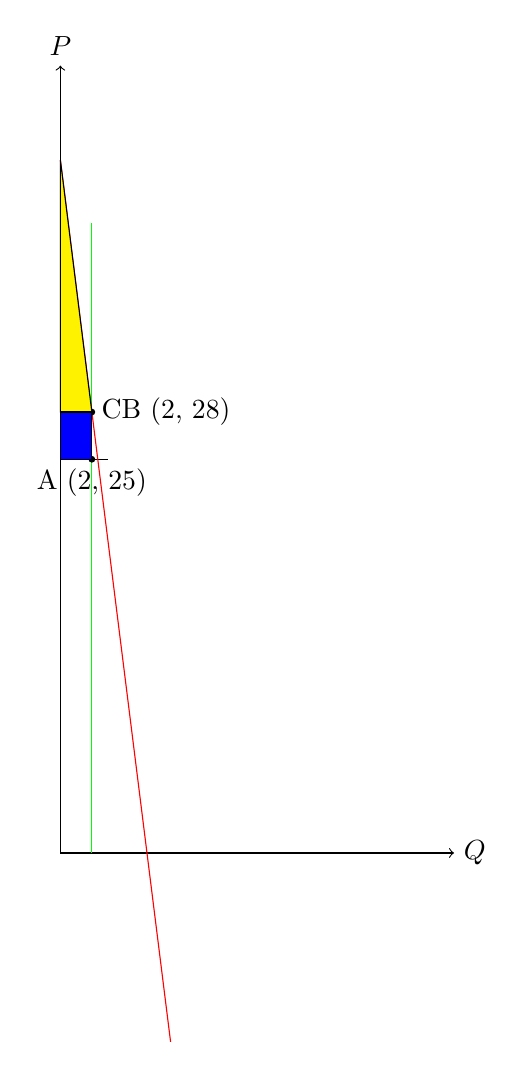
\begin{tikzpicture}
          \draw [->] (0,0) -- (5,0)node[right] {$Q$};
          \draw [->] (0,0) -- (0,10)node[above] {$P$};
          \draw [-, scale = 0.2, color=green] (2,0) -- (2,40);
          \draw [-, scale = 0.2, color=black] (0,25) -- (3,25);
          \draw[scale = 0.2, domain=0:7, smooth, variable=\x, color=red]
          plot ({\x}, {44 - 8 * \x});
          \filldraw[scale = 0.2, color=black] (2, 28)
          circle (5pt) node[anchor=west]{CB (2, 28)};
          \filldraw[scale = 0.2, color=black] (2, 25)
          circle (5pt) node[anchor=north]{A (2, 25)};

          \filldraw[fill=yellow, scale = 0.2] (0,28) -- (2,28) -- (0, 44) -- cycle;
          \filldraw[fill=blue, scale = 0.2] (0,28) -- (2,28) -- (2, 25) -- (0, 25) -- cycle;
        \end{tikzpicture}



    tại mức giá này CS = (44 - 28) * 2 / 2 + 2 * (28 - 25) = 16 + 6 = 22 và PS vẫn không xác định

\end{enumerate}

\section{Cung và cầu của hàng hóa X có phương trình như sau:}

$Q_D = 150 - 5P$ và $Q_S = 5P - 10$

\begin{enumerate}[a.]
  \item Tính giá và lượng cân bằng trên thị trường.
  
  $150 - 5P = 5P - 10$\\
  $10P = 160 \Rightarrow P = 16 \Rightarrow Q = 70$

  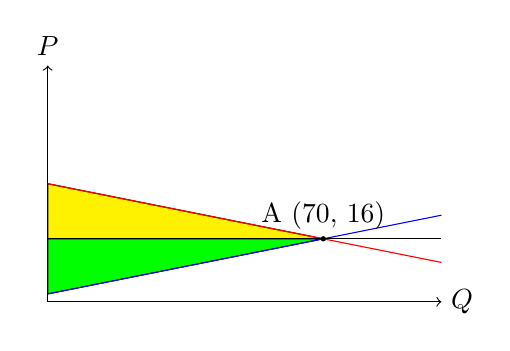
\begin{tikzpicture}
    \draw [->] (0,0) -- (5,0)node[right] {$Q$};
    \draw [->] (0,0) -- (0,3)node[above] {$P$};

    \filldraw[fill=yellow, scale = 0.05] (0,16) -- (70,16) -- (0, 30) -- cycle;
    \filldraw[fill=green, scale = 0.05] (0,16) -- (70,16) -- (0, 2) -- cycle;

    \draw[scale = 0.05, domain=0:100, smooth, variable=\x, color=red]
    plot ({\x}, {30 - \x / 5});
    \draw[scale = 0.05, domain=0:100, smooth, variable=\x, color=blue]
    plot ({\x}, {\x / 5 + 2});
    
    \filldraw[scale = 0.05, color=black] (70, 16)
    circle (15pt) node[anchor=south]{A (70, 16)};

    \draw [-, scale = 0.05, color=black] (0,16) -- (100,16);
   
    
 

  \end{tikzpicture}

  \item Nếu giá bán trên thị trường là P = 18 thì điều gì xảy ra trên thị trường? 
  
   hiện tượng dư cung, dư thừa hàng hóa xảy ra
  
  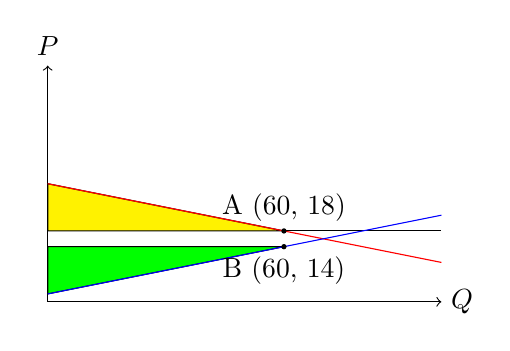
\begin{tikzpicture}
    \draw [->] (0,0) -- (5,0)node[right] {$Q$};
    \draw [->] (0,0) -- (0,3)node[above] {$P$};

    \draw [-, scale = 0.05, color=black] (0,18) -- (100,18);
    \filldraw[fill=yellow, scale = 0.05] (0,18) -- (60,18) -- (0, 30) -- cycle;
    \filldraw[fill=green, scale = 0.05] (0,14) -- (60,14) -- (0, 2) -- cycle;

    \draw[scale = 0.05, domain=0:100, smooth, variable=\x, color=red]
    plot ({\x}, {30 - \x / 5});
    \draw[scale = 0.05, domain=0:100, smooth, variable=\x, color=blue]
    plot ({\x}, {\x / 5 + 2});
    
    \filldraw[scale = 0.05, color=black] (60, 14)
    circle (15pt) node[anchor=north]{B (60, 14)};
    \filldraw[scale = 0.05, color=black] (60, 18)
    circle (15pt) node[anchor=south]{A (60, 18)};

   
  \end{tikzpicture}

  \item So sánh thặng dư sản xuất và thặng dư tiêu dùng tại trạng thái cân bằng và khi P = 18
  
   tại trạng thái cân bằng,\\
    CS = (30 - 16) * 70 / 2 = 14 * 35 \\
    PS = (16 - 2) * 70 / 2 = 14 * 35 \\
  tại P = 18 \\
  CS = (30 - 18) * 60 / 2 = 12 * 30 \\
  PS = (14 - 2) * 60 / 2 = 12 * 30 \\
  

\end{enumerate}

\section{Hàm cầu và hàm cung của trứng gà như sau:}

$P_D = 10 - Q$ và $ P_S = Q - 4$ \\
(P tình bằng nghìn đồng/1 quả, Q tính bằng triệu quả)


\begin{enumerate}[a.]
  \item .Tính giá và sản lượng cân bằng trên thị trường. Tính hệ số co giãn của cung và cầu tại
        mức giá cân bằng.

        chúng ta có $P_D = 10 - Q$ và $ P_S = Q - 4$ \\
        $10 -Q = Q - 4 \Rightarrow Q = 7, P = 3 $ là giá và sản lượng cân bằng

        chúng ta có công thức tính hệ số co giãn của cầu như sau
        \[ E_{DP} = \frac{\%\Delta Q_D}{\%\Delta P} =
          \frac{\Delta Q_D}{\Delta P} \times \frac{P}{Q_D} = Q_D' \times \frac{P}{Q_D} \]

        $Q_D' = ( 10 - P)' = -1$ \\
        vậy $E_{DP} = (-1) * 3 / 7 = -0.428 $

        chúng ta có công thức tính hệ số co giãn của cung như sau
        \[ E_{SP} = \frac{\%\Delta Q_S}{\%\Delta P} =
          \frac{\Delta Q_S}{\Delta P} \times \frac{P}{Q_S} = Q_S' \times \frac{P}{Q_S} \]

        $Q_S' = ( 4 + P)' = 1$ \\
        vậy $E_{SP} = (1) * 3 / 7 = 0.428 $

  \item Tính thặng dư sản xuất và thặng dư tiêu dùng tại mức giá cân bằng.
        chúng ta cần vẽ hình ra để dễ nhìn hơn

        CS = (10 - 3) * (7 - 0) / 2 = 49 / 2\\
        PS = ( 3 - (-4))  * (7 - 0) / 2 = 49 / 2\\

        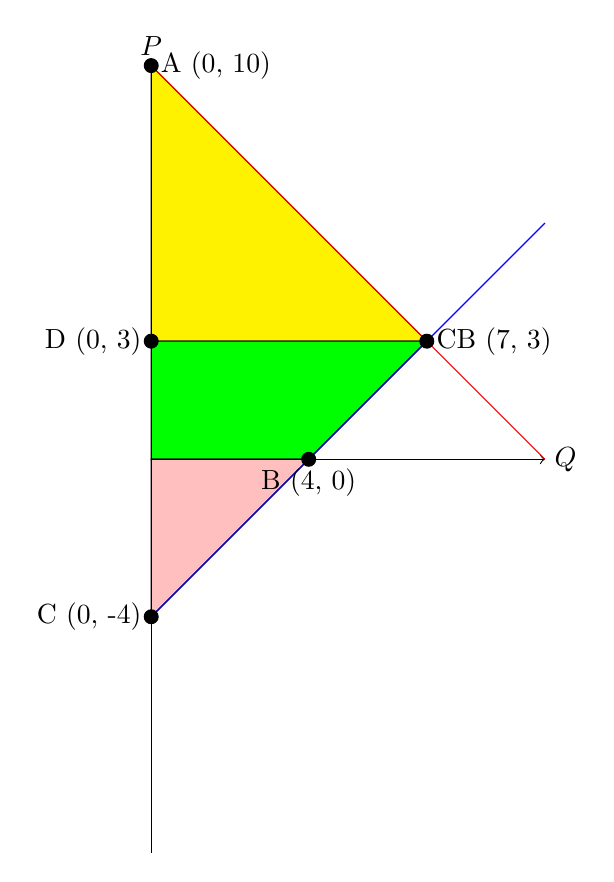
\begin{tikzpicture}
          \draw [->] (0,0) -- (5,0)node[right] {$Q$};
          \draw [->] (0,-5) -- (0,5)node[above] {$P$};

          \filldraw[fill=yellow, scale = 0.5] (0,3) -- (7,3) -- (0, 10) -- cycle;
          \filldraw[fill=green, scale = 0.5] (0,3) -- (7,3) -- (4, 0) -- (0, 0) -- cycle;
          \filldraw[fill=pink, scale = 0.5] (0,-4) --  (4, 0) -- (0, 0) -- cycle;

          \draw[scale = 0.5, domain=0:10, smooth, variable=\x, color=red]
          plot ({\x}, {10 - \x});
          \draw[scale = 0.5, domain=0:10, smooth, variable=\x, color=blue]
          plot ({\x}, {\x - 4});

          \filldraw[scale = 0.5, color=black] (7, 3)
          circle (5pt) node[anchor=west]{CB (7, 3)};
          \filldraw[scale = 0.5, color=black] (0, 10)
          circle (5pt) node[anchor=west]{A (0, 10)};
          \filldraw[scale = 0.5, color=black] (4, 0)
          circle (5pt) node[anchor=north]{B (4, 0)};

          \filldraw[scale = 0.5, color=black] (0, -4)
          circle (5pt) node[anchor=east]{C (0, -4)};

          \filldraw[scale = 0.5, color=black] (0, 3)
          circle (5pt) node[anchor=east]{D (0, 3)};

          %\draw [-, scale = 0.05, color=black] (0,16) -- (100,16);




        \end{tikzpicture}

  \item Khi giá bán trên thị trường P= 2 nghìn đồng/quả. Thặng dư sản xuất và thặng dư tiêu
        dùng thay đổi như thế nào so với trước?

        CS = (10 - 4) * (6 - 0) / 2 = 18\\
        PS = ( 2 - (-4))  * (6 - 0) / 2 = 18\\

        kết luận: thặng du sản xuất PS giảm, thặng dư tiêu dùng CS giảm

        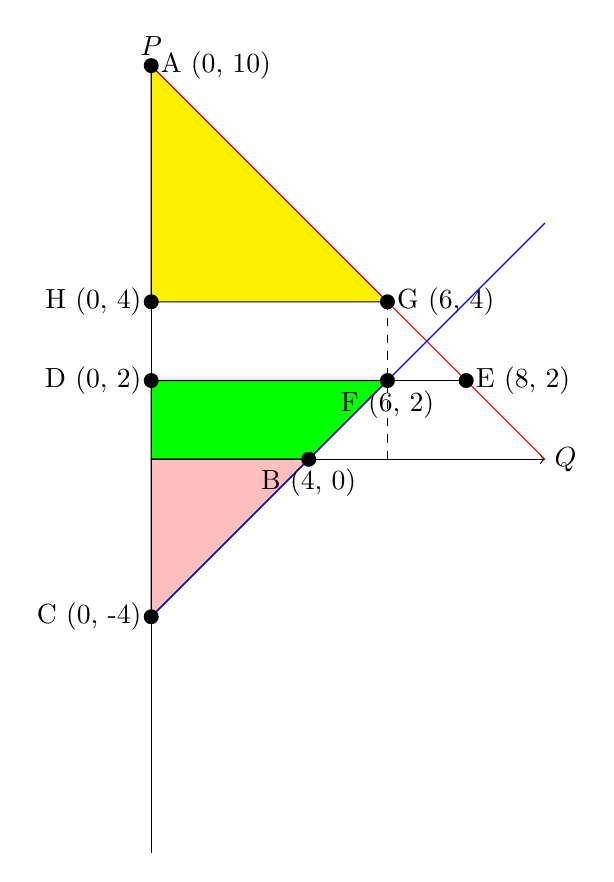
\begin{tikzpicture}
          \draw [->] (0,0) -- (5,0)node[right] {$Q$};
          \draw [->] (0,-5) -- (0,5)node[above] {$P$};

          \filldraw[fill=yellow, scale = 0.5] (0,4) -- (6,4) -- (0, 10) -- cycle;
          \filldraw[fill=green, scale = 0.5] (0,2) -- (6,2) -- (4, 0) -- (0, 0) -- cycle;
          \filldraw[fill=pink, scale = 0.5] (0,-4) --  (4, 0) -- (0, 0) -- cycle;
          %\filldraw[fill=olive, scale = 0.5] (0,3) -- (7,3) -- (8, 2) -- (0, 2) -- cycle;

          \draw[scale = 0.5, domain=0:10, smooth, variable=\x, color=red]
          plot ({\x}, {10 - \x});
          \draw[scale = 0.5, domain=0:10, smooth, variable=\x, color=blue]
          plot ({\x}, {\x - 4});
          \draw [dashed, scale = 0.5] (6,0) -- (6,4);
          

          \filldraw[scale = 0.5, color=black] (8, 2)
          circle (5pt) node[anchor=west]{E (8, 2)};
          \filldraw[scale = 0.5, color=black] (0, 10)
          circle (5pt) node[anchor=west]{A (0, 10)};
          \filldraw[scale = 0.5, color=black] (4, 0)
          circle (5pt) node[anchor=north]{B (4, 0)};

          \filldraw[scale = 0.5, color=black] (0, -4)
          circle (5pt) node[anchor=east]{C (0, -4)};

          \filldraw[scale = 0.5, color=black] (0, 2)
          circle (5pt) node[anchor=east]{D (0, 2)};
          \filldraw[scale = 0.5, color=black] (6, 2)
          circle (5pt) node[anchor=north]{F (6, 2)};
          \filldraw[scale = 0.5, color=black] (6, 4)
          circle (5pt) node[anchor=west]{G (6, 4)};
          \filldraw[scale = 0.5, color=black] (0, 4)
          circle (5pt) node[anchor=east]{H (0, 4)};

          \draw [-, scale = 0.5, color=black] (0,2) -- (8, 2);

        \end{tikzpicture}

\end{enumerate}